\section{Model Analysis}

A Monte Carlo simulation was run on three parameters of the model, and three inputs were gathered, as listed in figure 1. It was additionally assumed that only one technology is used for the duration of the search. Extension into multiple technologies is fully possible, but was not done during this Monte Carlo simulation in order to isolate the general search dynamics.

\begin{figure}[H]\begin{center}\begin{tabular}{|c|c|c|c|}
\hline \textbf{Parameter} & \textbf{Description} & \textbf{Minimum} & \textbf{Maximum}\\\hline\hline
$\alpha$ & Probability of success of one search & 0.2 & 0.5 \\\hline
$i$ & Number of search iterations performed & 10 & 750 \\\hline
$n_t$ & Number of ships used in search & 1 & 30 \\\hline\hline
\textbf{Output} & \textbf{Description} &&\\\hline
$DT$ & Total distance traveled by all ships &&\\\hline
$PS$ & Probability that the search has discovered the object &&\\\hline
$NS$ & Total number of searched cells &&\\\hline
$CT$ & Computation time for model (in ms) &&\\\hline
\end{tabular}\end{center}
\caption{Table of parameters and collected outputs.}
\end{figure}

In order to fully observe the dynamics of the search, all cell searches are assumed to have failed. This is simply a consequence of the fact that if the search had succeeded, it would have stopped. The goal is to observe dynamics.

The probability distribution used for input was intentionally designed to have several local maxima at varying heights. The probability distribution used is also continuous everywhere, though is not continuous past the first search iteration.

\begin{figure}[H]\begin{center}
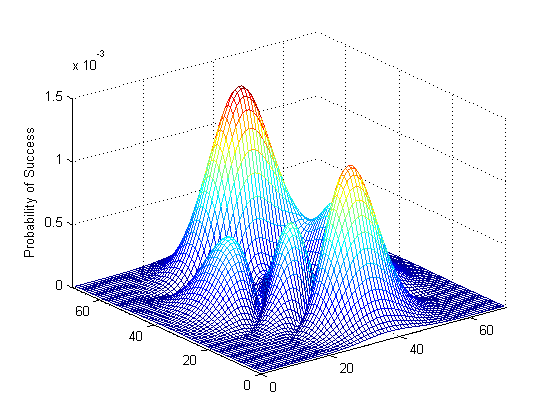
\includegraphics[scale=1]{..\Matlab\Images\InitialProbDist.png}
\end{center}\end{figure}